\newpage
\setcounter{section}{1}
\Section{Dataset 1: The UCI Breast Cancer Wisconsin}

In this Section, we will present the classification results of the first dataset that we used in our project, which is the UCI Breast Cancer Wisconsin dataset \cite{breast_cancer_wisconsin}.

The dataset contains features computed from a digitized image of a fine needle aspirate (FNA) of a breast mass. These features describe characteristics of the cell nuclei present in the image. A sample of such images can be found at \url{http://www.cs.wisc.edu/~street/images/}.

\subsubsection*{Dataset Characteristics}
\begin{itemize}
    \item \textbf{Type:} Multivariate
    \item \textbf{Subject Area:} Health and Medicine
    \item \textbf{Associated Task:} Classification
    \item \textbf{Feature Type:} Real-valued
    \item \textbf{Number of Instances:} 569
    \item \textbf{Number of Features:} 30
    \item \textbf{Missing Values:} No
\end{itemize}

\subsubsection*{Dataset Insights}
\begin{itemize}
    \item \textbf{Source:} Digitized images of fine needle aspirates (FNA) of breast masses.
    \item \textbf{Objective:} Classify tumors as malignant (M) or benign (B).
    \item \textbf{Methodology:} Features were computed using image analysis techniques to describe characteristics of cell nuclei.
    \item \textbf{Additional Details:}
    \begin{itemize}
        \item Separating planes were determined using the Multisurface Method-Tree (MSM-T).
        \item Feature selection involved exhaustive searches in feature and plane spaces.
    \end{itemize}
\end{itemize}

\subsubsection*{Feature Description}
\begin{itemize}
    \item \textbf{Input Variables:} Ten real-valued features computed for each cell nucleus:
    \begin{enumerate}
        \item \textbf{Radius:} Mean distance from the center to the perimeter.
        \item \textbf{Texture:} Standard deviation of gray-scale values.
        \item \textbf{Perimeter:} Measurement of the contour length.
        \item \textbf{Area:} Size of the cell nucleus.
        \item \textbf{Smoothness:} Local variation in radius lengths.
        \item \textbf{Compactness:} Computed as $(\text{perimeter}^2 / \text{area}) - 1.0$.
        \item \textbf{Concavity:} Severity of concave portions of the contour.
        \item \textbf{Concave Points:} Number of concave portions of the contour.
        \item \textbf{Symmetry:} Symmetry of the cell nucleus.
        \item \textbf{Fractal Dimension:} Approximation of the contour's fractal nature.
    \end{enumerate}
    \item \textbf{Output Variable:}
    \begin{itemize}
        \item Diagnosis: Binary classification where M = malignant and B = benign.
    \end{itemize}
\end{itemize}
\subsection{Data preparation}

\subsubsection{Import the dataset}

The \href{https://archive.ics.uci.edu/}{UC Irvine Machine Learning Repository} allows for direct dataset import in Python using the \texttt{ucimlrepo} package. The package is included in the \texttt{requirements.txt} file. The following code demonstrates how to import the Breast Cancer Wisconsin (id = 17) dataset using the \texttt{fetch\_ucirepo} function:

\lstset{style=code}
\begin{lstlisting}[language=Python]
from ucimlrepo import fetch_ucirepo 

breast_cancer_wisconsin_diagnostic = fetch_ucirepo(id=17) 
    
X = breast_cancer_wisconsin_diagnostic.data.features 
y = breast_cancer_wisconsin_diagnostic.data.targets 
\end{lstlisting}

\subsubsection{Splitting the dataset}

The dataset is split into training and testing sets using the \texttt{train\_test\_split} function from the \texttt{sklearn} library. 
The dataset is splitted into 4 sets of different test sizes: 60\%, 40\%, 20\%, and 10\% of the dataset in stratified fashion, using the random state of 22125 to ensure reproducibility.

\begin{figure}[H]
    \centering
    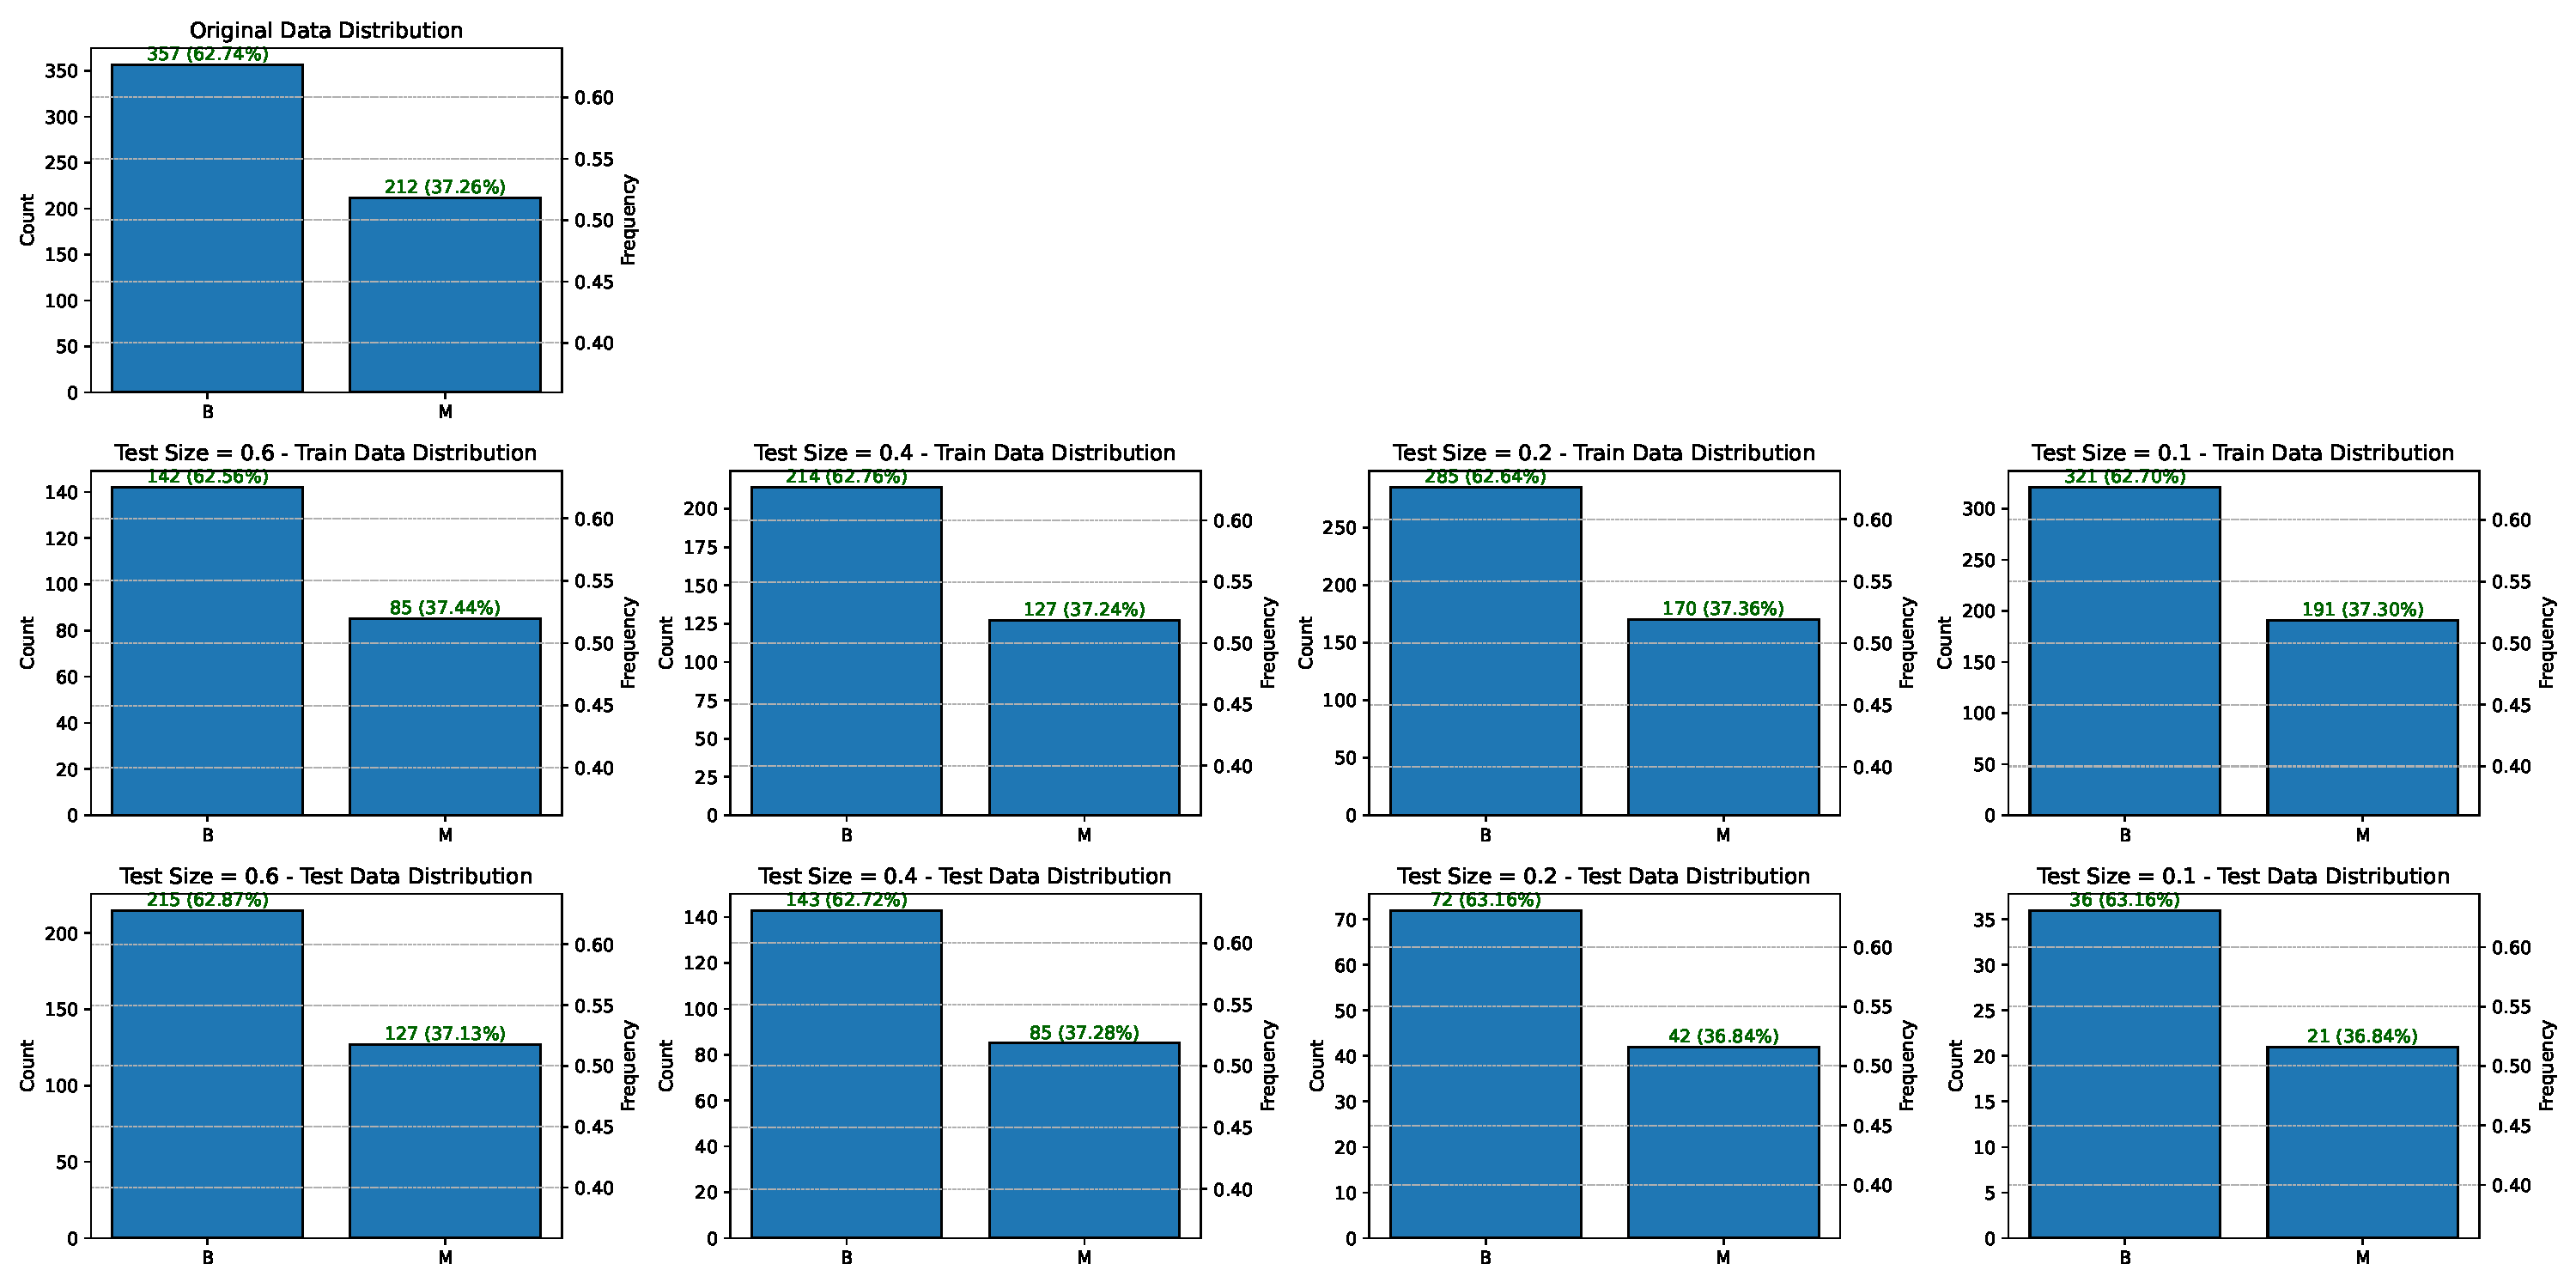
\includegraphics[width=\textwidth]{figures/breast_cancer_wisconsin_split.pdf}
    \caption{Breast Cancer Wisconsin dataset split}
    \label{fig:breast_cancer_wisconsin_split}
\end{figure}

As shown in figure \ref{fig:breast_cancer_wisconsin_split}, the distribution of the target class is preserved in all splits.

\subsection{Decision Tree classifier implementation}

Decision Tree classifiers are implemented using the \texttt{DecisionTreeClassifier} class from the \texttt{sklearn} library. 
To ensure reproducibility, the random state is set to 22125. 
We use the Entropy (information gain) criterion to split the nodes and set the maximum depth of the tree to None to allow the tree to grow until all leaves are pure.

\begin{figure}[H]
    \centering
    \includegraphics[width=\textwidth]{figures/breast_cancer_wisconsin_decision_trees.pdf}
    \caption{Breast Cancer Wisconsin dataset Decision Trees with different test sizes}
    \label{fig:breast_cancer_wisconsin_decision_trees}
\end{figure}

The Decision Trees are visualized in figure \ref{fig:breast_cancer_wisconsin_decision_trees}. The trees grow deeper as the test size decreases, indicating that the model is more complex and overfits the training data when the test size is small.

The first node of the Decision Tree splits the dataset based on different features:
\begin{itemize}
    \item Decision tree of test size 60\% chooses the feature \texttt{concave\_points3} to split the dataset.
    \item Decision tree of test size 40\% and 20\% chooses the feature \texttt{area3} to split the dataset.
    \item Decision tree of test size 10\% chooses the feature \texttt{perimeter3} to split the dataset.
\end{itemize}

Despite the differences in the splitting features, the first node's entropy is approximately 0.953 in all Decision Trees, indicating that the first split is not very informative. However, the Decision Tree classifier effectively splits the dataset into pure leaves with high information gain.

\subsection{Performance evaluation}

\subsubsection{Classification report}

The classification report provides a comprehensive evaluation of the Decision Tree classifier's performance using the \texttt{classification\_report} function from the \texttt{sklearn.metrics} module. The report includes the following metrics:
\begin{itemize}
    \item \textbf{Precision:} The ratio of true positive samples to the sum of true positive and false positive samples.
    \item \textbf{Recall:} The ratio of true positive samples to the sum of true positive and false negative samples.
    \item \textbf{F1-score:} The harmonic mean of precision and recall.
    \item \textbf{Support:} The number of samples in each class.
\end{itemize}

\textbf{Classification Report for Test Size = 0.6}

\begin{tabular}{lcccccc}
\hline
 & \textbf{Precision} & \textbf{Recall} & \textbf{F1-score} & \textbf{Support} \\
\hline
B & 0.94 & 0.94 & 0.94 & 215 \\
M & 0.90 & 0.89 & 0.89 & 127 \\
\hline
\textbf{Accuracy} & & & 0.92 & 342 \\
\textbf{Macro avg} & 0.92 & 0.91 & 0.92 & 342 \\
\textbf{Weighted avg} & 0.92 & 0.92 & 0.92 & 342 \\
\hline
\end{tabular}

\vspace{2em}

\textbf{Classification Report for Test Size = 0.4}

\begin{tabular}{lcccccc}
\hline
 & \textbf{Precision} & \textbf{Recall} & \textbf{F1-score} & \textbf{Support} \\
\hline
B & 0.94 & 0.92 & 0.93 & 143 \\
M & 0.87 & 0.89 & 0.88 & 85 \\
\hline
\textbf{Accuracy} & & & 0.91 & 228 \\
\textbf{Macro avg} & 0.91 & 0.91 & 0.90 & 228 \\
\textbf{Weighted avg} & 0.91 & 0.91 & 0.91 & 228 \\
\hline
\end{tabular}

\vspace{2em}

\textbf{Classification Report for Test Size = 0.2}

\begin{tabular}{lcccccc}
\hline
 & \textbf{Precision} & \textbf{Recall} & \textbf{F1-score} & \textbf{Support} \\
\hline
B & 0.95 & 0.88 & 0.91 & 72 \\
M & 0.81 & 0.93 & 0.87 & 42 \\
\hline
\textbf{Accuracy} & & & 0.89 & 114 \\
\textbf{Macro avg} & 0.89 & 0.90 & 0.88 & 114 \\
\textbf{Weighted avg} & 0.90 & 0.89 & 0.90 & 114 \\
\hline
\end{tabular}

\vspace{100em}

\textbf{Classification Report for Test Size = 0.1}

\begin{tabular}{lcccccc}
\hline
 & \textbf{Precision} & \textbf{Recall} & \textbf{F1-score} & \textbf{Support} \\
\hline
B & 0.97 & 0.92 & 0.94 & 36 \\
M & 0.87 & 0.95 & 0.91 & 21 \\
\hline
\textbf{Accuracy} & & & 0.93 & 57 \\
\textbf{Macro avg} & 0.93 & 0.93 & 0.92 & 57 \\
\textbf{Weighted avg} & 0.93 & 0.93 & 0.93 & 57 \\
\hline
\end{tabular}

The classification reports show that the Decision Tree classifier performs well on the Breast Cancer Wisconsin dataset, achieving an accuracy of 92\% for the test size of 60\%, 91\% for the test size of 40\%, 89\% for the test size of 20\%, and 93\% for the test size of 10\%. The classifier has high precision, recall, and F1-score for both classes, indicating that it effectively distinguishes between malignant and benign samples.

Prediction performance is better for the benign class, with higher precision, recall, and F1-scores across all test sizes, likely due to the dataset's imbalance favoring benign samples.
\subsubsection{Confusion matrix}

The confusion matrix provides a visual representation of the Decision Tree classifier's performance using the \texttt{confusion\_matrix} function from the \texttt{sklearn.metrics} module. The matrix shows the number of true positive, false positive, true negative, and false negative samples for each class.

\begin{figure}[H]
    \centering
    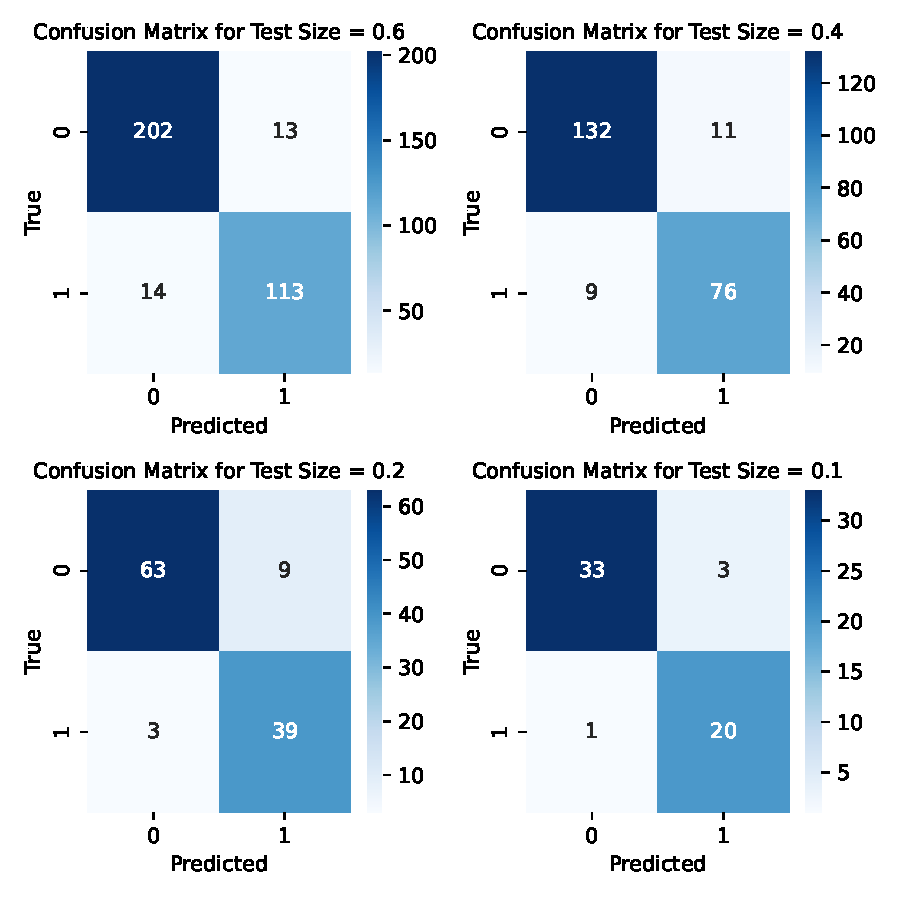
\includegraphics[width=.7\textwidth]{figures/breast_cancer_wisconsin_confusion_matrices.pdf}
    \caption{Breast Cancer Wisconsin dataset Confusion Matrices with different test sizes}
    \label{fig:breast_cancer_wisconsin_confusion_matrices}
\end{figure}
% Confusion Matrix for Test Size = 0.6:
% [[202  13]
%  [ 14 113]]
% Confusion Matrix for Test Size = 0.4:
% [[132  11]
%  [  9  76]]
% Confusion Matrix for Test Size = 0.2:
% [[63  9]
%  [ 3 39]]
% Confusion Matrix for Test Size = 0.1:
% [[33  3]
%  [ 1 20]]

The confusion matrices in figure \ref{fig:breast_cancer_wisconsin_confusion_matrices} show that the Decision Tree classifier correctly classifies most samples in the Breast Cancer Wisconsin dataset. The number of false positive and false negative samples is low, indicating that the classifier has high precision and recall for both classes.

\subsection{Depth vs Accuracy evaluation}

The Decision Tree classifier's performance is evaluated by varying the maximum depth of the tree. The accuracy of the classifier is computed for different maximum depths using the \texttt{accuracy\_score} function from the \texttt{sklearn.metrics} module for the Decision Tree classifier with a test size of 20\%.

\begin{table}[H]
    \centering
    \begin{tabular}{|l|c|c|c|c|c|c|c|}
        \hline
        \textbf{\texttt{max\_depth}} & None & 2 & 3 & 4 & 5 & 6 & 7 \\ \hline
        \textbf{Accuracy} & 0.89 & 0.89 & 0.93 & 0.89 & 0.87 & 0.89 & 0.89 \\ \hline
    \end{tabular}
    \caption{Breast Cancer Wisconsin dataset Depth vs Accuracy}
    \label{tab:breast_cancer_wisconsin_depth_vs_accuracy}
\end{table}

The table \ref{tab:breast_cancer_wisconsin_depth_vs_accuracy} shows that the Decision Tree classifier achieves the highest accuracy on the test data when the maximum depth of the tree is 3. The accuracy decreases as the maximum depth increases, indicating that the model overfits the training data when the tree is too deep.

\begin{figure}[H]
    \centering
    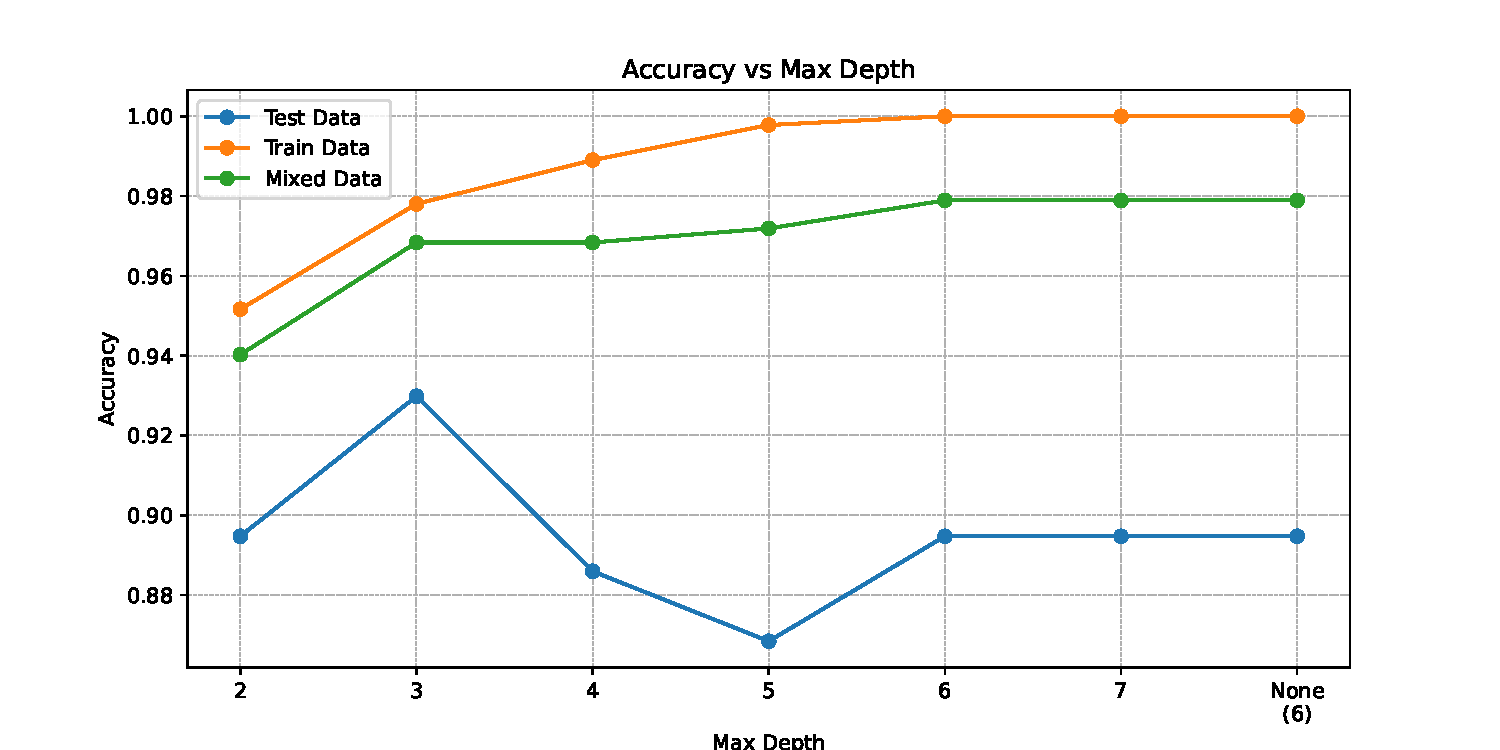
\includegraphics[width=\textwidth]{figures/breast_cancer_wisconsin_accuracy_vs_max_depth.pdf}
    \caption{Breast Cancer Wisconsin dataset Depth vs Accuracy}
    \label{fig:breast_cancer_wisconsin_depth_vs_accuracy}
\end{figure}

The plot in figure \ref{fig:breast_cancer_wisconsin_depth_vs_accuracy} supports the findings in table \ref{tab:breast_cancer_wisconsin_depth_vs_accuracy}.
